\section{Gates}

\qs{Double control gate}
{
    Verify the equivalence of the two following circuits:
    \begin{center}
        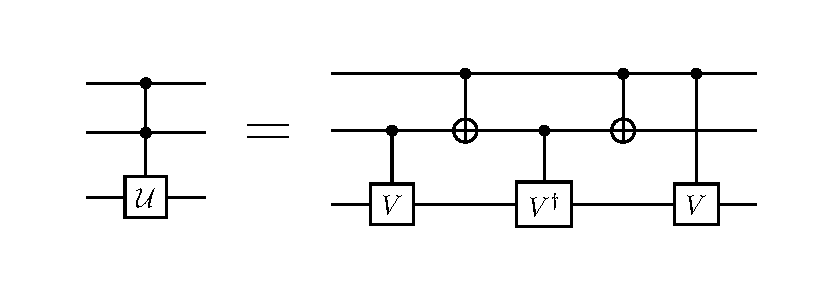
\includegraphics[width=0.7\textwidth]{Immagini/CCU.pdf}
    \end{center}
    Where the unitary operation $V$ is defined as $\sqrt{\mathcal{U}}$.
}
\pf{Solution}
{
    Two main ways of soliving this problem can be used, the first and simplest one is by constructing the thruth table of the two circuits and see that is the same. Something that is left to the reader since it's a really simple task. The other one is by going with a matrix multiplication and seing how the matrix form of the circuit on the right is the same as the general double control. To see that first we can write the following form of the matrix of the circuit
    \begin{equation}
        \left( CV_{13}\otimes\mathbb{1}_2 \right)\left( CNOT_{12}\otimes \mathbb{1}_3 \right)\left( \mathbb{1}_1\otimes CV^\dagger_{23} \right)\left( CNOT_{12}\otimes \mathbb{1}_3 \right)\left( \mathbb{1}_1 \otimes CV_{23} \right).
    \end{equation}
    Now, we know how to write down the majority of those matrices but one. For example, we can easily write the following thing
    \begin{equation}
        \mathbb{1}_1\otimes CV^\dagger_{23} = \begin{pmatrix}
            1 & 0\\
            0 & 1
        \end{pmatrix}\otimes\begin{pmatrix}
            \mathbb{1} & \mathbb{0}\\
            \mathbb{0} & V
        \end{pmatrix} = \begin{pmatrix}
            \mathbb{1} & \mathbb{0} & \mathbb{0} & \mathbb{0}\\
            \mathbb{0} & V & \mathbb{0} & \mathbb{0}\\
            \mathbb{0} & \mathbb{0} & \mathbb{1} & \mathbb{0}\\
            \mathbb{0} & \mathbb{0} & \mathbb{0} & V\\
        \end{pmatrix},
    \end{equation}
    where the tensor product rule has been used in the multiplication. Still, a problem is present in the evaluation of the first matrix, because the order matters in tensor product and in that case the control is applied to a qubit that is not directly attached to the one of the target. Therefore, the main way we have to evaluate that matrix is to swap the qubit and then use a normal control gate as we have seen right now
    \begin{equation}
        CV_{13}\otimes\mathbb{1}_2 = \left( S_{12}\otimes\mathbb{1}_3 \right)\left( \mathbb{1}_1 \otimes CV_{23} \right)\left( S_{12}\otimes\mathbb{1}_3 \right).
    \end{equation}
    By recalling the form of the swap operator matrix being \eqref{eq:swapMatrix} we can perform now all the computation to obtain
    \begin{equation}
        CV_{13}\otimes\mathbb{1}_2 = \begin{pmatrix}
            \mathbb{1} & \mathbb{0} & \mathbb{0} & \mathbb{0}\\
            \mathbb{0} & \mathbb{1} & \mathbb{0} & \mathbb{0}\\
            \mathbb{0} & \mathbb{0} & V & \mathbb{0}\\
            \mathbb{0} & \mathbb{0} & \mathbb{0} & V\\
        \end{pmatrix},
    \end{equation}
    which then can be used to perform the matrix multiplication and obtain the final form of the gate that wuold be analogous to the one of a CCU gate.
}